\clearpage
\subsubsection{USB-B}
\label{subsubsec:USB-B}

Im Folgenden wird der in Kapitel \ref{subsec:USB-B} erwähnte USB-Anschluss beschrieben. Es handelt sich dabei um einen USB-UART-Converter mit zugehöriger Beschaltung wie z.B USB-B-Buchse, ESD-Schutz und weitere passive Komponenten.

\paragraph{Schema}\mbox{}

Auf dem Schema ist die USB-Buchse mit J2 gekennzeichnet. Der dazugehörige ESD-Schutz bildet die Diodenschaltung D2-4. Der Converter hat die Bezeichnung IC2. Die Widerstände R12 und R13 bilden einen Spannungsteiler, welcher an die 5V-Eingangsspannung der Buchse und an dem VBUS-Eingang des Converters hängt. Die Widerstände R16, R19, R10 und R11 reduzieren den Kurzschlussstrom zwischen dem USB-UART-Converter und dem ESP32. Der Widerstand R14 ist ein Pull-Up Widerstand, welcher verhindert, dass der Reset-Pin einen ungewünschten Zustand annimmt. Die Widerstände R17 und R18 reduzieren den Strom durch die LED's.

\begin{figure}[h!]
	\centering
	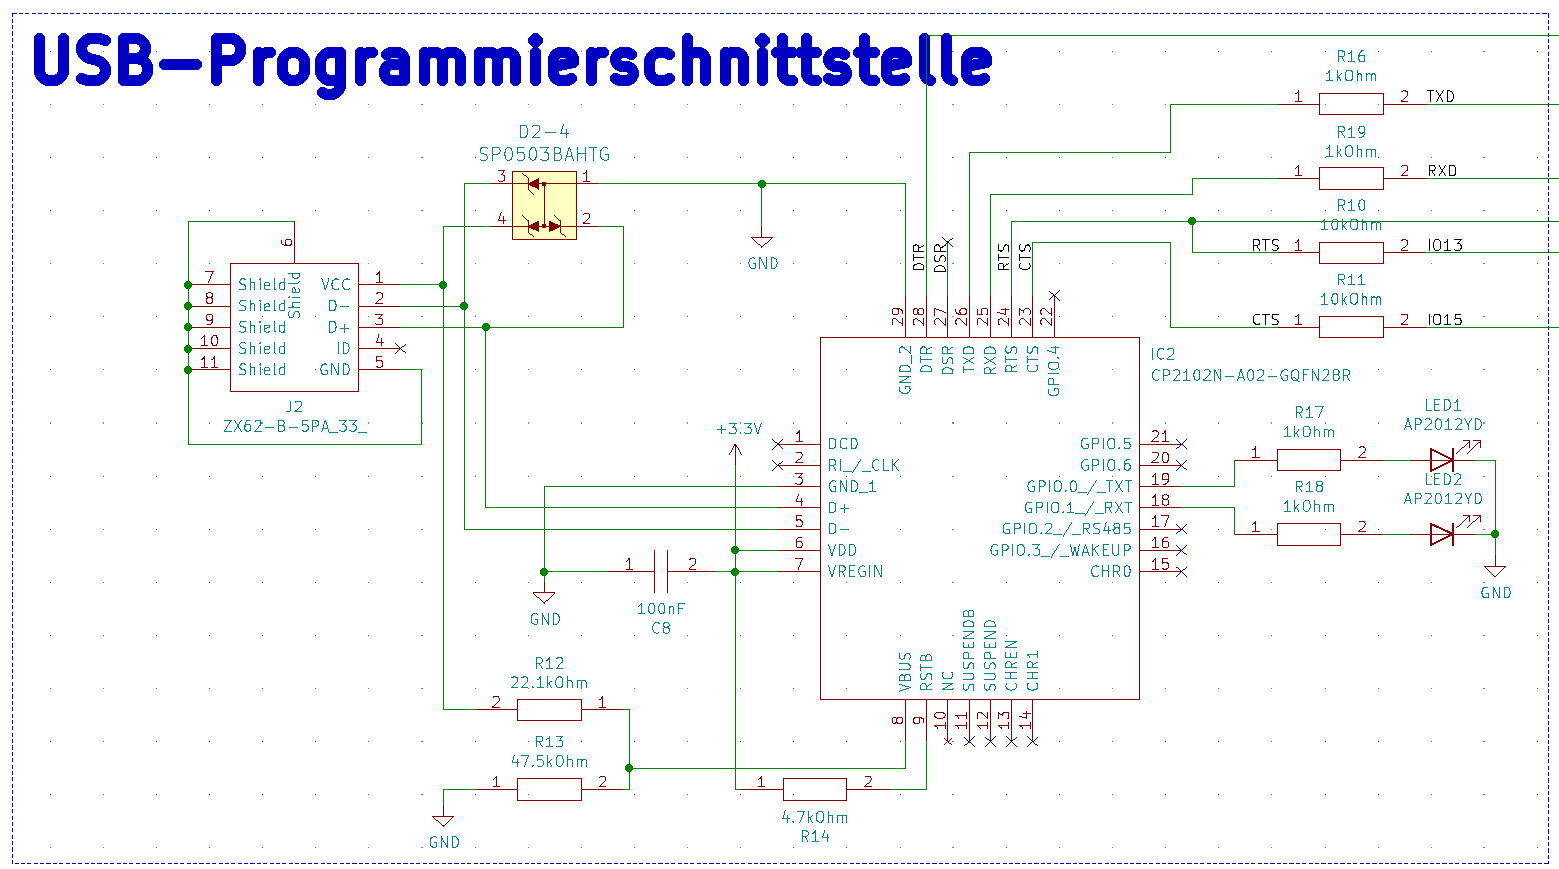
\includegraphics[width=1\textwidth]{graphics/Schema_USB_B}
	\caption{Schema USB-B.}
	\label{fig:Schema_USB_B}
\end{figure}

\paragraph{Funktionsbeschrieb der Schaltung}\mbox{}

Sobald ein USB-Kabel vom PC zum Converter angeschlossen wird, liegt 5V am Spannungsteiler, was vom IC als bestehende Netzwerk-Verbindung interpretiert wird. Die USB-Kommunikation zwischen PC und Converter findet über die Leitungsn D+ und D- statt. Aufgrund des differentielen Verfahrens und Verwendung von verdrillten Drähten werden Störungen von ausserhalb zu einem grossen Teil eliminiert. Der Vorteil der asynchronen serielle Schnittstelle (UART) zeigt sich im Falle der Cocktailmaschine vor allem im flexiblem Protokoll und dem einfach zu implementierenden Handshake, welcher benutzt wird, um in den Boot-Modus der Empfänger (ATMega2560 und ESP32) zu gelangen. Die LED's zeigen an, wenn eine Kommunikation stattfindet. Die Widerstände in den Kommunikations- und Steuerleitungen schützen die Pins vor hohen Strömen im Falle von Spannungsunterschieden.